\documentclass{standalone}
\usepackage{pgfplots}
\pgfplotsset{compat=1.18}
\usepgfplotslibrary{fillbetween}
\renewcommand{\familydefault}{\sfdefault}

\definecolor{myDarkGray}{gray}{0.3}  
\definecolor{myMidGray}{gray}{0.55}   
\definecolor{myLightGray}{gray}{0.75}  
% kommentiere jeweils den Block aus, der nicht gebraucht wird

% Graustufen
% \definecolor{myDarkGray}{gray}{0.3}  
% \definecolor{myMidGray}{gray}{0.55}   
% \definecolor{myLightGray}{gray}{0.75}


% Farben
\colorlet{myDarkGray}{blue} 
\colorlet{myMidGray}{orange}
\colorlet{myLightGray}{green}

\begin{document}
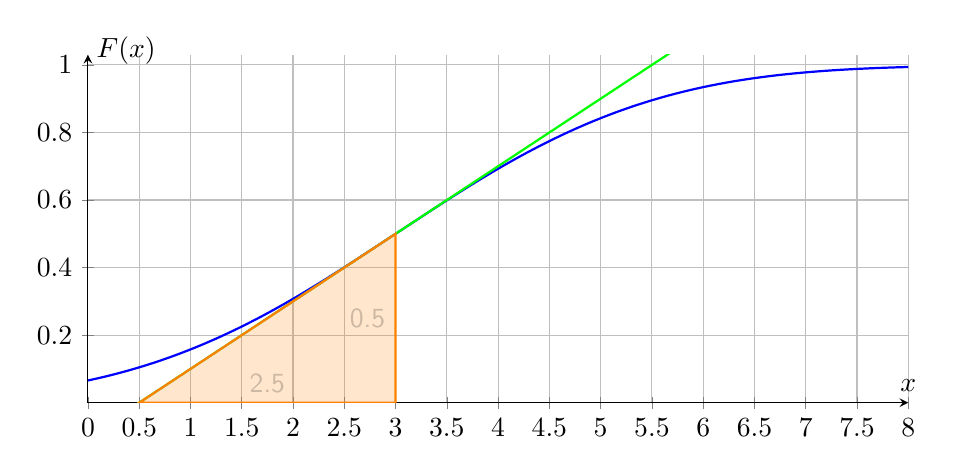
\begin{tikzpicture}
\pgfmathdeclarefunction{erf}{1}{%
  \pgfmathparse{sign(#1)*(1 - 1/(1 + 0.278393*abs(#1) + 0.230389*abs(#1)^2 + 0.000972*abs(#1)^3 + 0.078108*abs(#1)^4)^4)}%
}
\begin{axis}[
    xlabel={$x$},
    ylabel={$F(x)$},
    grid=major,
    width=12cm,
    height=6cm,
    ymin=0, ymax=1.03,
    ytick={0.2,0.4,...,1},
    xmin=0, xmax=8,
    xtick={0,0.5,...,8},
    axis lines=left,
    xlabel style={at={(ticklabel* cs:1)}, anchor=north, yshift=12pt},
    ylabel style={
        at={(ticklabel* cs:1)}, 
        anchor=north east,
        rotate=-90, 
        xshift=28pt,
        yshift=10pt}
]

\addplot [
    domain=0:8, 
    samples=100, 
    color=myDarkGray, 
    thick
] {0.5*(1 + erf((x-3)/(1.99*sqrt(2))))};

%Tangente
\addplot[
    domain=0:8,
    samples=100,
    color=myLightGray,
    thick
] {(0.5/2.5)*(x-3)+0.5};

%Steigungsdreieck
\filldraw[thick, draw=myMidGray, fill=myMidGray, fill opacity=0.2] 
    (axis cs:0.5,0) 
    -- node[above, pos=0.5] {2.5}
    (axis cs:3,0) 
    -- node[left, pos=0.5] {0.5}
    (axis cs:3,0.5) -- cycle;


\end{axis}
\end{tikzpicture}
\end{document}